Die Methode der Diffusion beobachtet, wie sich ein Stoff im Schnee ausbreitet. Für den Vorversuch wurde der Schnee unter ein Stereo-Mikroskop platziert. Der Versuch dauert etliche Minuten. Um zu verhindern, dass der Schnee von der warmen Raumluft aufgeschmolzen wird, ist der Schnee in einer Röhre aus Eis platziert. Während das -10 Grad Celsius kalte Eis langsam schmilzt, kann der Versuch durchgeführt werden. Die Auswertung bei dem Vorversuch erfolgt visuell, indem beobachtet wird, wie sich blaue Tinte im Schnee ausbreitet.

Eine Kombination dieses Ansatzes mit der Leitfähigkeitsmessung (siehe \ref{sec:Volt}) ist möglich, wenn ein leitfähiger Stoff eingesetzt wird.

Ich vermute, dass dieser Ansatz von der Geometrie des Schnees beeinflusst wird. Wieviel flüssiges Wasser vorhanden ist, ist sekundär zu wie die Eiskristalle miteinander verbunden sind.

\begin{figure}[H]
    \centering
    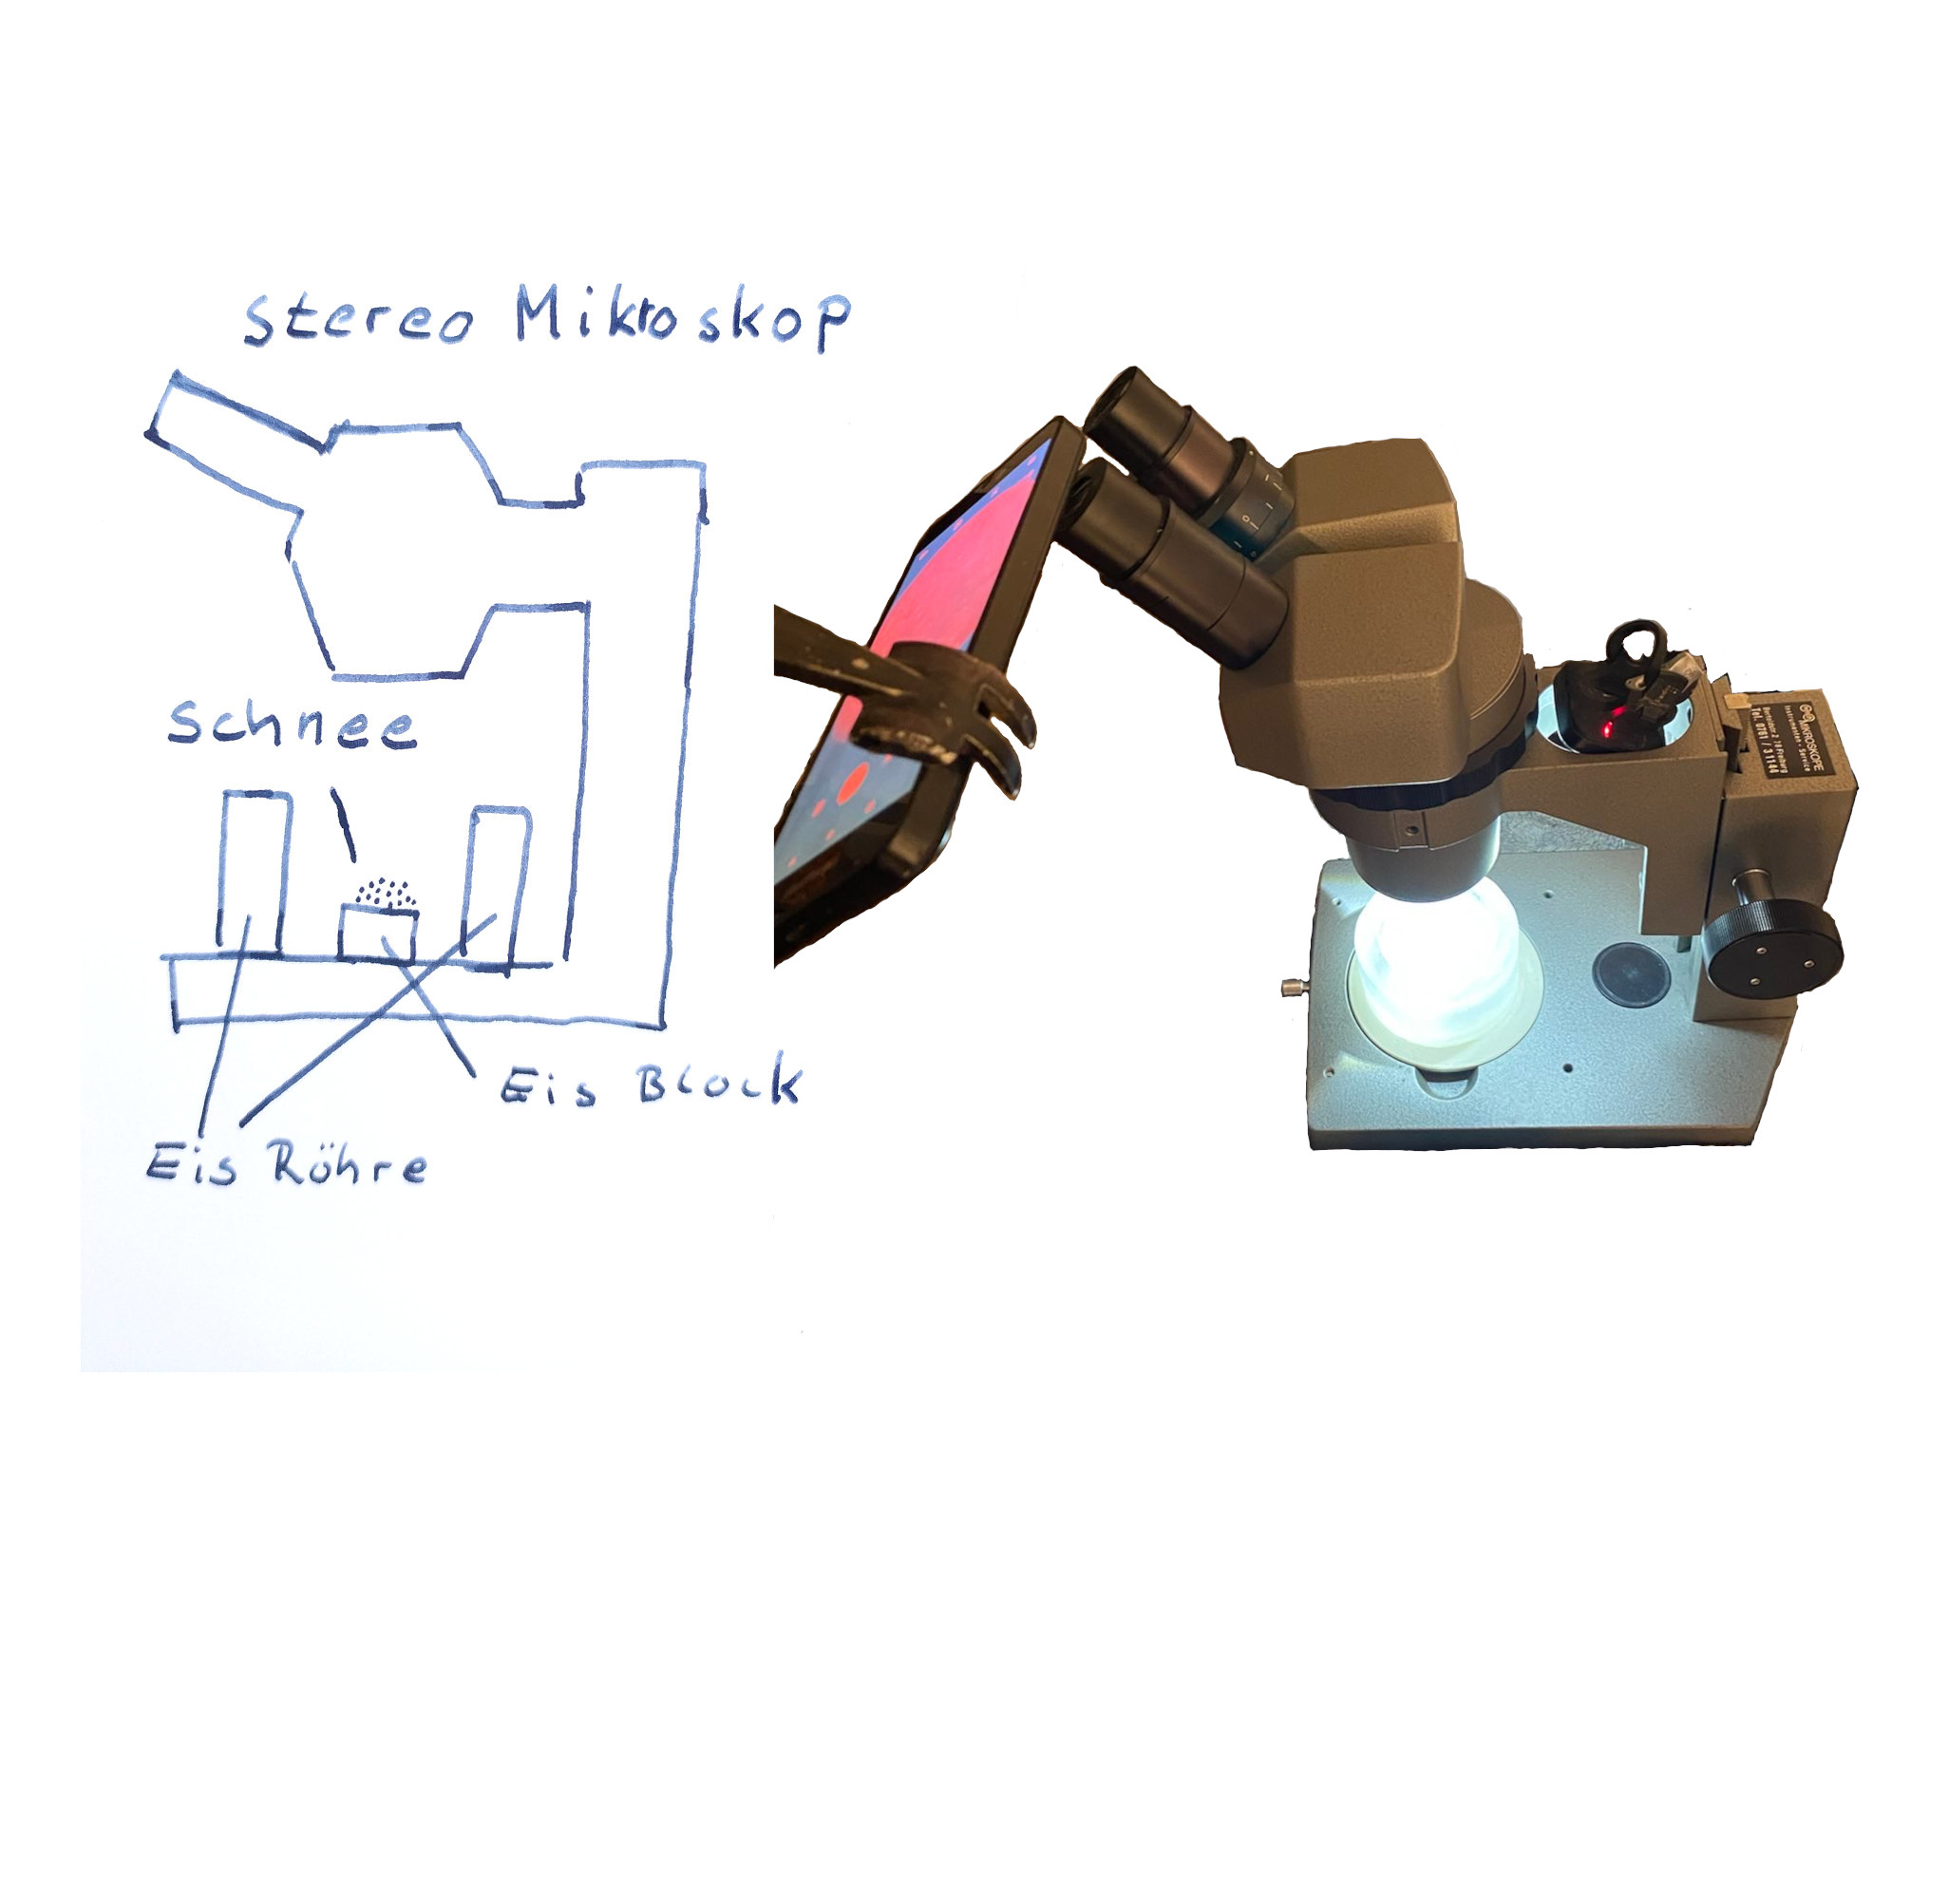
\includegraphics[width=0.8\textwidth]{Bilder/freistellen.jpeg}
    \caption{Aufbau einer Messung wo der Schnee durch eine Eis Röhre gekühlt wird}
    \label{fig:AutMess}
\end{figure}
